\documentclass[11pt]{beamer}
\usepackage[UTF8,scheme=plain]{ctex}
\usepackage{listings}
\usepackage[utf8]{inputenc}
\usepackage[T1]{fontenc}
\usepackage{amsmath}
\usepackage{amsfonts}
\usepackage{amssymb}
\usepackage{graphicx}
\usetheme{Boadilla}

\usepackage{framed} % 可以用 \begin{shaded},即背景色块
\definecolor{shadecolor}{rgb}{0.9,0.9,0.9}

\newcommand{\kong}[1][0.5]{\vspace{#1cm}}

\begin{document}
	\author{ 路毅 \hspace{0.3cm} 曲阜师范大学 }
	\date{\number\year 年 \number\month 月 \number\day 日}
	\title{数学物理方法第八章}

\begin{frame}
	\maketitle
\end{frame}

\kaishu

\begin{frame}{第八章:热传导方程的傅里叶解}
\begin{itemize}
	\item 第一节:热传导方程和扩散方程的建立
	\vspace{1cm}
	\item 第二节:混合问题的傅里叶解
	\vspace{1cm}
	\item 第三节:初值问题的傅里叶解
	\vspace{1cm}
	\item 第四节:一端有界的热传导问题	
\end{itemize}
\end{frame}

\begin{frame}{热传导方程}
如图均匀细长杆,热量在上面传导,记$u(x,t)$为$x$点$t$时刻的温度。
\begin{figure}
\centering
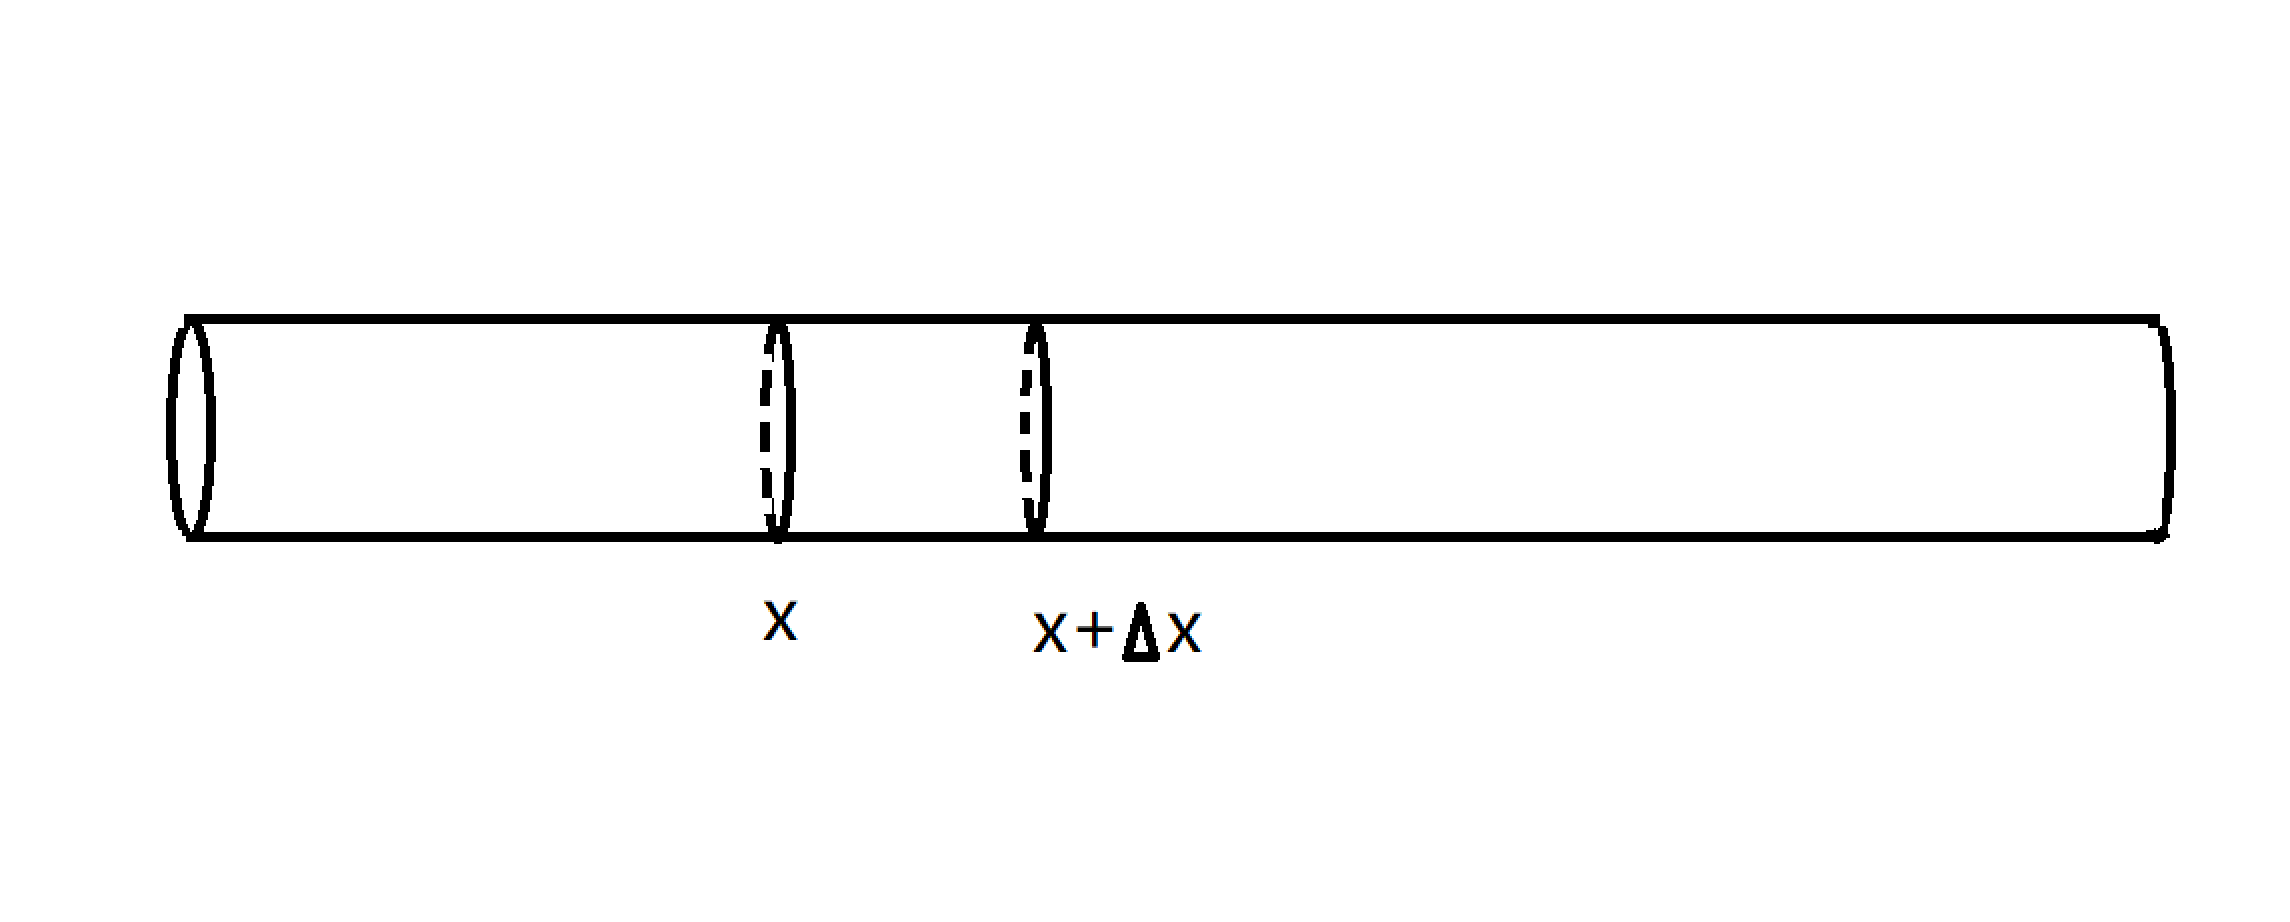
\includegraphics[width=0.7\linewidth]{chap8扩散方程}
\end{figure}
取$[x,x+\Delta x]$小段,$\Delta t$内从$x$左端流入区间内的热量为
\begin{equation}
\Delta Q_1 = -k u_x (x,t) A \Delta t,
\end{equation}
其中$k>0$为导热系数,$A$为细杆横截面积,这个方程是由实验定律决定的:传热速度与温度梯度$u_x$成正比。
\end{frame}

\begin{frame}{热传导方程}
$\Delta t$内从$x+\Delta x$右侧传入区间的热量为
\begin{equation}
\Delta Q_2 = k u_x(x+\Delta x, t) A \Delta t,
\end{equation}
所以$\Delta t$内净流入热量为
\begin{equation}
\Delta Q_1 + \Delta Q_2 = k \Delta x A \Delta t u_{xx}(x,t),
\end{equation}
上式利用了$\Delta x$充分小,$u_x(x+\Delta x, t) - u_x(x,t) \rightarrow u_{xx}(x,t) \Delta x$。

流入的热量会使得$[x,x+\Delta x]$区间内的温度上升,即
\begin{equation}
\Delta Q_1 + \Delta Q_2 = c \rho A \Delta x u_t \Delta t,
\end{equation}
上式中$c$为热容,$\rho$为密度,故$\rho A \Delta x$为这一小段材料的质量。

所以有
\begin{equation}
k A u_{xx} \Delta x \Delta t = c \rho A u_t \Delta x \Delta t,
\end{equation}
\end{frame}

\begin{frame}{热传导方程}
即
\begin{equation}
c \rho u_t = k u_{xx},
\end{equation}
可写作
\begin{equation}
u_t = a^2 u_{xx}, ~~ a^2 = \frac{k}{c\rho},
\end{equation}
这就是热传导方程。\\

\kong[0.5]
如果细杆内存在热源(比如:电烙铁,或者“热得快”),即$\Delta t$内传入$[x,x+\Delta x]$内的热量还需加上$F(x,t)\Delta x \Delta t$,其中$F(x,t)$为热源单位时间单位长度产热。
即
\begin{equation}
k A u_{xx} \Delta x \Delta t + F(x,t)\Delta x \Delta t = c \rho A u_t \Delta x \Delta t,
\end{equation}
得到
\begin{equation}
u_t = a^2 u_{xx} + f, ~~ f=\frac{F}{c \rho A},
\end{equation}

\end{frame}

\begin{frame}{一维扩散方程}
\begin{figure}
\centering
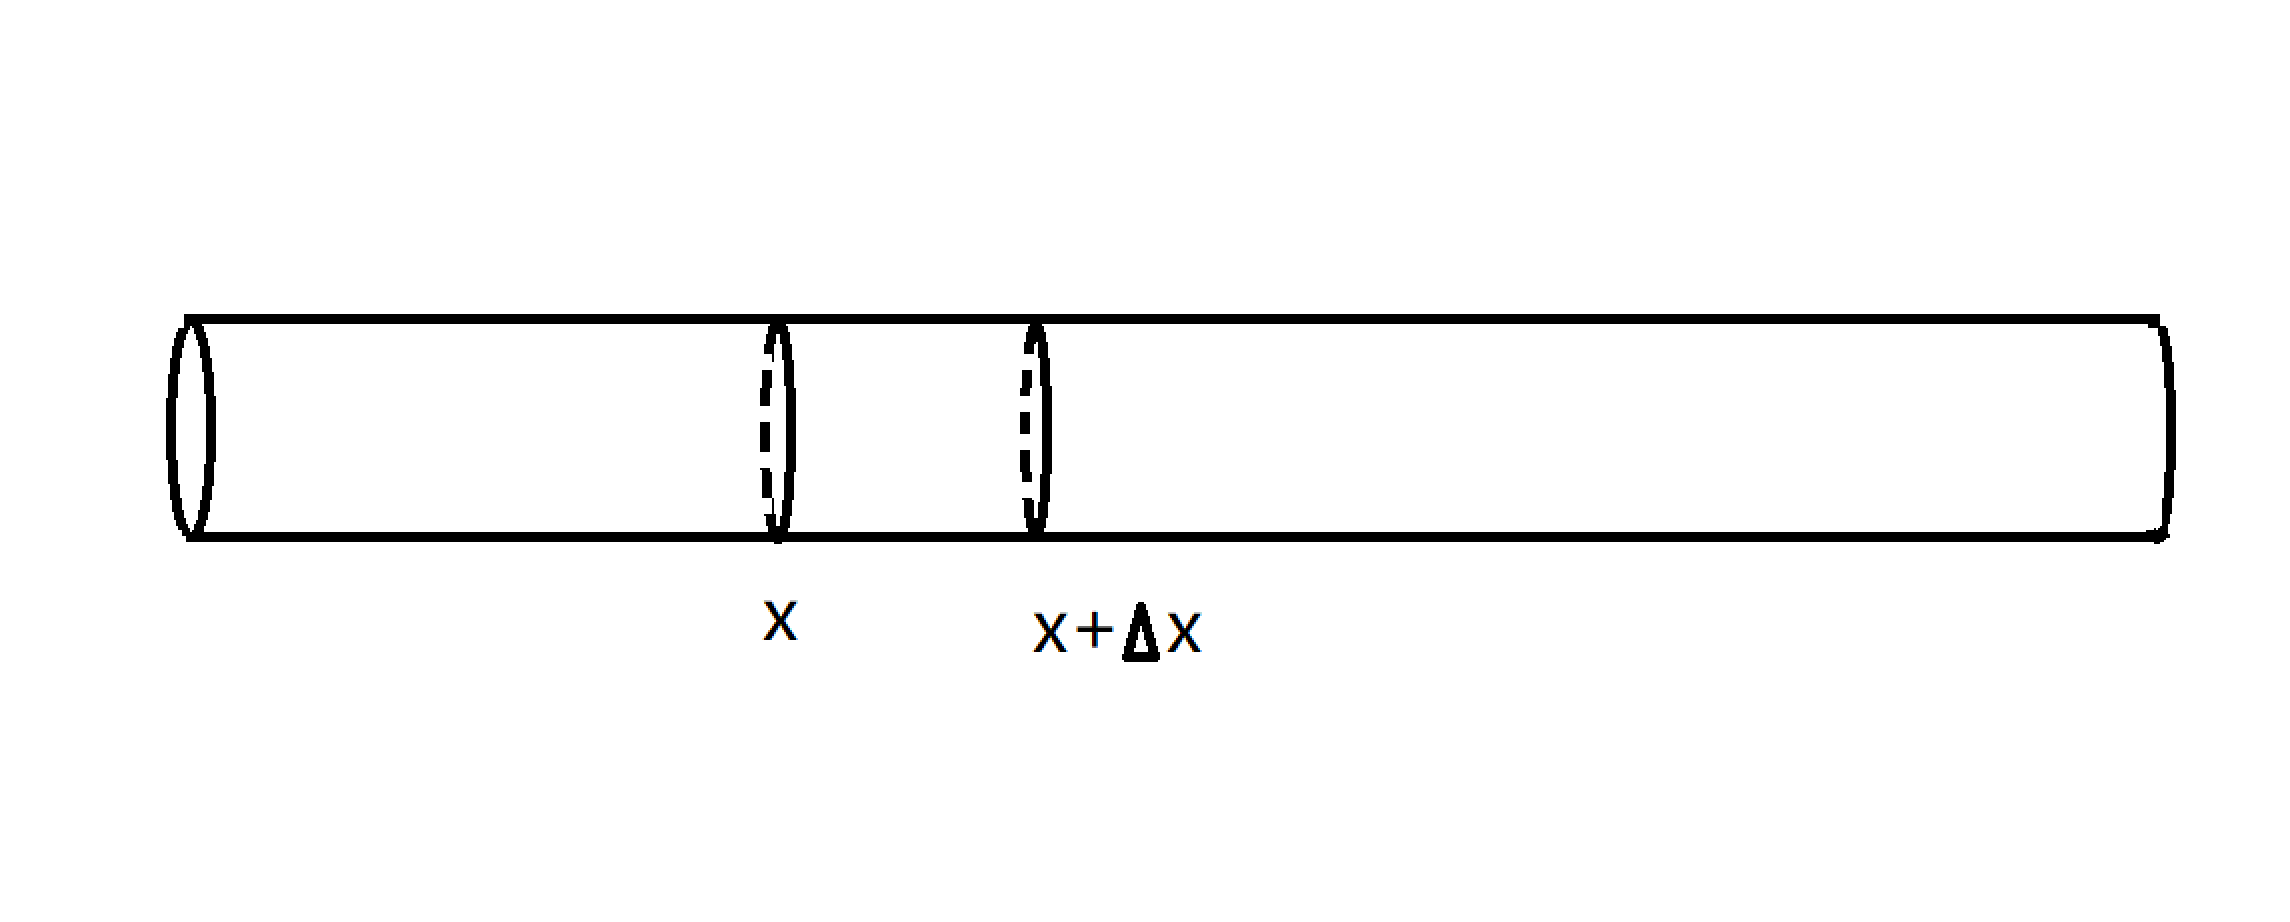
\includegraphics[width=0.7\linewidth]{chap8扩散方程}
\end{figure}
如图所示,考虑一根细杆上,杂质在材料中的扩散。
用$N(x,t)$表示$x$处在时间$t$的杂质质量密度,即杂质浓度。

取小区间$[x,x+\Delta x]$,$\Delta t$内从$x$左侧扩散进入$[x,x+\Delta x]$的杂质质量为
\begin{equation}
\Delta m_1 = - D N_x(x,t) A \Delta t,
\end{equation}
其中$D$称为扩散系数,$A$是横截面积,上式是实验定律决定的:扩散快慢与浓度梯度成正比。
\end{frame}

\begin{frame}{一维扩散方程}
$\Delta t$内从$[x,x+\Delta x]$右侧传入的杂质质量为
\begin{equation}
\Delta m_2 = D N_x(x+\Delta x, t) A \Delta t,
\end{equation}
所以,$\Delta t$内净流入质量为
\begin{equation}
\Delta m_1 + \Delta m_2 = D( N_x(x+\Delta x, t) - N_x(x,t) ) A \Delta t
= D N_{xx}(x,t) \Delta x A \Delta t,
\end{equation}
上式利用了$\Delta x$充分小这一点:$N_x(x+\Delta x, t) - N_x(x,t) \rightarrow N_{xx}(x,t) \Delta x$。

流入的杂质使得区间内浓度上升
\begin{equation}
D N_{xx} A \Delta x \Delta t = N_t \Delta t A \Delta x,
\end{equation}
得到
\begin{equation}
N_t = a^2 N_{xx}, a^2 = D.
\end{equation}
\end{frame}

\begin{frame}{热量传导 v.s. 杂质扩散}
热量传导:传导快慢正比于温度梯度。

\kong[0.3]
杂质扩散:扩散快慢正比于浓度梯度。

\kong[0.3]
因为物理规律的相似,这两种物理过程都由同一种数学形式来表达
\begin{equation}
u_t = a^2 u_{xx}.
\end{equation}

\kong[0.3]
热量传导,可以看作是热量的扩散。
\end{frame}

\begin{frame}{热传导方程定解条件}
热传导方程:
\begin{equation}
u_{t} = a^2 u_{xx},
\end{equation}
初始条件:初始时刻杆上的温度分布$\varphi(x)$。

边界条件的三种情况(以右端点为例):
\begin{itemize}
\item 已知端点温度 $u(l,t) = \mu(t)$。
\item 已知端点单位截面单位时间流出的热量 $\nu(t)$,则根据傅里叶实验定律(温差越大,导热越快),有
\begin{equation}
\nu(t) A = - k u_x (l, t) A,
\end{equation}
即
\begin{equation}
u_x (l,t) = - \frac{1}{k} \nu(t).
\end{equation}
\item 端点与介质接触,该介质温度已知为$\theta(t)$,则单位时间流出热量
\begin{equation}
- k u_x(l,t) A = h( u(l,t) - \theta(t) ) A,
\end{equation}
上式右侧为关于热交换的牛顿实验定律(温差越大,导热越快)。所以有
\begin{equation}
k u_x (l,t) + h u(l,t) = h \theta(t).
\end{equation}
\end{itemize}

\end{frame}

\begin{frame}{混合问题的傅里叶解:两端温度恒为0}
\begin{equation}
\left\{
\begin{aligned}
u_t = a^2 u_{xx}, (0<x<l, t>0) \\
u(0,t) =0, u(l,t) = 0, (t \geq 0) \\
u(x,0) = \varphi(x), (0 \leq x \leq l)
\end{aligned}
\right.
\end{equation}
杆两端泡在冰水中,所以温度恒为0,初始时刻杆上有一定温度分布。

\kong[0.5]
如果杆是烧红的铁棒,那么热量会迅速流向冰水中,铁棒上的温度逐渐下降,直到变成一根冰冷的铁棒。

\kong[0.5]
如果杆是刚从液氮中取出,极其寒冷,那么热量会迅速从冰水中流向铁棒,温暖它,直到它变成0度的铁棒。
\end{frame}

\begin{frame}{分离变量法}
故技重施,我们先设一个简单的形式
\begin{equation}
u(x,t) = T(t) X(x),
\end{equation}
代入$u_t = a^2 u_{xx}$,得到
\begin{equation}
\frac{1}{a^2} \frac{T'}{T} = \frac{X''}{X} = - \lambda,
\end{equation}
求解
\begin{equation}
\left\{
\begin{aligned}
X''/X = - \lambda, \\
X(0) = X(l) = 0,
\end{aligned}
\right.
\end{equation}
得到(上式中$X(0)=X(l)=0$是由$u(0,t)=u(l,t)=0$推得),
\begin{equation}
\lambda_n = \frac{n^2 \pi^2}{l^2}, n=1,2,3,\cdots
\end{equation}
\end{frame}

\begin{frame}{分离变量法}
相应地,
\begin{equation}
X_n(x) = \sin \frac{n\pi x}{l}, ~~ T_n (t) = C_n e^{-a^2 \lambda_n t},
\end{equation}
即
\begin{equation}
u_n(x,t) = C_n e^{-a^2 \lambda_n t} \sin \frac{n\pi x}{l}.
\end{equation}
所有$u_n(x,t)$叠加起来,得到
\begin{equation}
u(x,t) = \sum^\infty_{n=1} C_n e^{-a^2 \lambda_n t} \sin \frac{n\pi x}{l}.
\end{equation}
取$t=0$,得到
\begin{equation}
u(x,0) = \sum^\infty_{n=1} C_n \sin \frac{n\pi x}{l} = \varphi(x).
\end{equation}
即
\begin{equation}
C_n = \frac{2}{l} \int^l_0 \varphi(x) \sin \frac{n\pi x}{l} dx, n=1,2,3,\cdots
\end{equation}
{\tiny 只要$\varphi(x)$满足狄利克雷条件(物理问题中都满足),上面的$C_n$代入$u(x,0)$,就一定会在任意$x$收敛至$\varphi(x)$。}
\end{frame}

\begin{frame}{$l \rightarrow \infty$:傅里叶级数$\rightarrow$傅里叶积分}
使用有限的$l$值,傅里叶级数的一般形式为
\begin{equation}
f(x) = \frac{a_0}{2} + \sum^\infty_{n=1} ( a_n \cos \frac{n\pi x}{l} + b_n \sin \frac{n\pi x}{l} ),
\end{equation}
其中$a_n, b_n$为
\begin{eqnarray}
&& a_n \equiv \frac{1}{l} \int^l_{-l} f(\xi) \cos \frac{n \pi \xi}{l} d \xi, n=0,1,2,\cdots \\
&& b_n \equiv \frac{1}{l} \int^l_{-l} f(\xi) \sin \frac{n \pi \xi}{l} d \xi, n=1,2,\cdots \\
\end{eqnarray}
将$a_n, b_n$代入上面的$f(x)$式,得到
\begin{equation}
f(x) = \frac{1}{2l} \int^l_{-l} f(x) dx + \sum^\infty_{n=1} \frac{1}{l}\int^l_{-l} f(\xi) \cos \frac{n\pi(\xi - x)}{l} d \xi.
\end{equation}
上式使用了差角公式$\cos \frac{n\pi(\xi - x)}{l} = \cos \frac{n\pi\xi}{l} \cos \frac{n\pi x}{l} + \sin \frac{n\pi\xi }{l} \sin \frac{n\pi x}{l}$。
\end{frame}

\begin{frame}{$l \rightarrow \infty$:傅里叶级数$\rightarrow$傅里叶积分}

如果$\int^\infty_{-\infty} |f(x)| dx$有限,即绝对可积,那么可取$l \rightarrow \infty$极限,
\begin{equation}
f(x) = \lim\limits_{l \rightarrow \infty} \sum^\infty_{n=1} \frac{1}{l} \int^l_{-l} f(\xi) \cos \frac{n \pi (\xi - x)}{l} d \xi.
\end{equation}
取$\lambda_1 = \frac{\pi}{l}, \lambda_2 = \frac{2\pi}{l}, \cdots, \Delta \lambda_n = \lambda_{n+1} - \lambda_n = \frac{\pi}{l}$,则有
\begin{eqnarray}
f(x) &=& \sum\limits^\infty_{n=1}\lim\limits_{\Delta \lambda \rightarrow 0} \frac{1}{\pi} \Delta \lambda \int^\infty_{-\infty} f(\xi) \cos( \lambda_n (\xi - x) ) d \xi \nonumber \\
&=& \frac{1}{\pi} \int^\infty_0 d \lambda \int^\infty_{-\infty} f(\xi) \cos(\lambda (\xi - x)) d \xi \nonumber \\
&=& \frac{1}{2\pi} \int^\infty_{-\infty} d \lambda \int^\infty_{-\infty} f(\xi) \cos(\lambda (\xi - x)) d \xi .
\end{eqnarray}

\end{frame}

\begin{frame}{$l \rightarrow \infty$:傅里叶级数$\rightarrow$傅里叶积分}
\begin{equation}
f(x) = \frac{1}{2\pi} \int^\infty_{-\infty} d \lambda \int^\infty_{-\infty} f(\xi) \cos(\lambda (\xi - x)) d \xi ,
\end{equation}
可以拆开,得到
\begin{equation}
f(x) = \int^\infty_{-\infty} [ A(\lambda) \cos(\lambda x) + B(\lambda) \sin(\lambda x)] d\lambda,
\end{equation}
其中
\begin{eqnarray}
&& A(\lambda) = \frac{1}{2\pi} \int^\infty_{-\infty} f(\xi) \cos(\lambda \xi) d \xi, \\
&& B(\lambda) = \frac{1}{2\pi} \int^\infty_{-\infty} f(\xi) \sin(\lambda \xi) d \xi.
\end{eqnarray}

\end{frame}

\begin{frame}{无穷长杆初值问题}
\begin{equation}
\left\{
\begin{aligned}
u_t = a^2 u_{xx}, (-\infty < x < \infty, t>0), \\
u(x,0) = \varphi(x), (-\infty < x < \infty),
\end{aligned}
\right.
\end{equation}
故技重施,先构造分离变量的解,$u(x,t) = T(t) X(x)$,然后再线性叠加,用初始条件约束得到问题的最终解。
\begin{equation}
\left\{
\begin{aligned}
T' + \lambda a^2 T = 0, \\
X'' + \lambda X = 0.
\end{aligned}
\right.
\end{equation}
$\lambda = 0$时,得到平庸解。

$\lambda <0$时,得到
\begin{equation}
X = A e^{\sqrt{-\lambda}x} + B e^{-\sqrt{-\lambda}x},
\end{equation}
在$\pm \infty$发散,是非物理的解。
\end{frame}

\begin{frame}{无穷长杆初值问题}
$\lambda >0$时,记$\mu^2 = \lambda$,则有
\begin{equation}
\left\{
\begin{aligned}
T' + \mu^2 a^2 T = 0, \\
X'' + \mu^2 X = 0.
\end{aligned}
\right.
\end{equation}
得到
\begin{equation}
\left\{
\begin{aligned}
X_\mu = A(\mu)\cos(\mu x) + B(\mu) \sin(\mu x), \\
T_\mu = e^{-\mu^2 a^2 t}
\end{aligned}
\right.
\end{equation}
即
\begin{equation}
u_\mu(x,t) = (A(\mu)\cos(\mu x) + B(\mu) \sin(\mu x))e^{-\mu^2 a^2 t}.
\end{equation}
通解形式为
\begin{equation}
u(x,t) = \int^\infty_{-\infty} u_\mu(x,t) d\mu = \int^\infty_{-\infty} (A(\mu)\cos(\mu x) + B(\mu)\sin(\mu x))e^{-\mu^2 a^2 t} d\mu.
\end{equation}
\end{frame}

\begin{frame}{无穷长杆初值问题}
在$t=0$时,有
\begin{equation}
u(x,0) = \int^\infty_{-\infty} u_\mu(x,0) d\mu = \int^\infty_{-\infty} (A(\mu)\cos(\mu x) + B(\mu)\sin(\mu x)) d \mu = \varphi(x),
\end{equation}
根据(39-41)式,即
\begin{eqnarray}
A(\mu) &=& \frac{1}{2\pi} \int^\infty_{-\infty} \varphi(\xi) \cos(\mu \xi) d \xi, \\
B(\mu) &=& \frac{1}{2\pi} \int^\infty_{-\infty} \varphi(\xi) \sin(\mu \xi) d \xi.
\end{eqnarray}
代入$u(x,t)$的表达式,即(48)式,得到

\end{frame}

\begin{frame}{无穷长杆初值问题}
\begin{eqnarray}
u(x,t) &=& \frac{1}{2\pi} \int^\infty_{-\infty} \int^\infty_{-\infty} \varphi(\xi) e^{-\mu^2 a^2 t} \cos(\mu(\xi-x)) d\xi d\mu \nonumber\\
&=& \frac{1}{2\pi} \int^\infty_{-\infty} \varphi(\xi) (\int^\infty_{-\infty} e^{-\mu^2 a^2 t} \cos(\mu(\xi-x)) d\mu) d\xi,
\end{eqnarray}

利用第五章课件中的泊松积分公式:
\begin{equation}
\int^\infty_0 e^{-ax^2} \cos(bx) dx = \frac{1}{2} \sqrt{\frac{\pi}{a}} e^{-\frac{b^2}{4a}},
\end{equation}
可知
\begin{equation}
\int^\infty_{-\infty} e^{-\mu^2 a^2 t} \cos(\mu(\xi-x)) d\mu = \frac{\sqrt{\pi}}{a \sqrt{t}} e^{- \frac{(\xi-x)^2}{4 a^2 t}}.
\end{equation}
所以有
\begin{equation}
u(x,t) = \frac{1}{2a\sqrt{\pi t}} \int^\infty_{-\infty} \varphi(\xi) e^{- \frac{(\xi-x)^2}{4a^2 t}} d\xi.
\end{equation}

\end{frame}

\begin{frame}{无限长杆初值问题傅里叶解的物理意义}
考虑点热源,即初始时杆上温度分布为
\begin{equation}
\psi(x) = \left\{
\begin{aligned}
&\varphi(x), &-\delta + x_0 < x < x_0 + \delta, \\
&0, &else
\end{aligned}
\right.
\end{equation}
其中$\delta$非常小。
代入(55)式,得到任意时刻温度分布
\begin{equation}
u(x,t) = \frac{1}{2a\sqrt{\pi t}} \varphi(x_0) 2\delta e^{- \frac{(x_0 - x)^2}{4a^2 t}},
\end{equation}
所以对任意$t$,$v(x,t)$呈正态分布,
随着$t$增大,$v(x,t)$的最大值减小,范围扩大,即热量扩散开来。

所以,初始温度分布为$\varphi(x)$时,$u(x,t)= \frac{1}{2a\sqrt{\pi t}} \int^\infty_{-\infty} \varphi(\xi) e^{- \frac{(\xi-x)^2}{4a^2 t}} d\xi$可做如下阐释:

初始温度分布$\varphi(x)$可以看做无限个小点源,每个点源向两边扩散热量,所有点源的热扩散总效果叠加,即时刻$t$的温度分布$u(x,t)$。
\end{frame}

\begin{frame}{无限长杆热传导:初始温度分布为奇函数}
在前文中,我们解决了如下问题
\begin{equation}
\left\{
\begin{aligned}
&& u_t = a^2 u_{xx}, ~~ ( -\infty < x < \infty, t>0) \\
&& u(x,0) = \varphi(x), ~~ ( -\infty <x< \infty ),
\end{aligned}
\right.
\end{equation}
上节已经得到傅里叶解
\begin{equation}
u(x,t) = \frac{1}{2a\sqrt{\pi t}} \int^\infty_{-\infty} \varphi(\xi) e^{ - \frac{(\xi - x)^2}{4a^2 t} } d \xi,
\end{equation}

1. 如果$\varphi(x)$是奇函数,则有
\begin{equation}
u(0,t) = \frac{1}{2a\sqrt{\pi t}} \int^\infty_{-\infty} \varphi(\xi) e^{ - \frac{(\xi)^2}{4a^2 t} } d \xi = 0,
\end{equation}
\end{frame}

\begin{frame}{无限长杆热传导:初始温度分布为偶函数}

2. 如果$\varphi(x)$是偶函数,则有
\begin{equation}
u_x(x,t) = \frac{1}{2a\sqrt{\pi t}} \int^\infty_{-\infty} \varphi(\xi) 
( - \frac{2(x-\xi)}{4a^2 t} )
e^{ - \frac{(\xi - x)^2}{4a^2 t} } d \xi,
\end{equation}
所以
\begin{equation}
u_x(0,t) = \frac{1}{2a\sqrt{\pi t}} \int^\infty_{-\infty} \varphi(\xi) 
( \frac{2\xi}{4a^2 t} )
e^{ - \frac{\xi^2}{4a^2 t} } d \xi = 0,
\end{equation}

\end{frame}

\begin{frame}{一端有界的热传导问题}
\begin{equation}
\left\{
\begin{aligned}
& u_t = a^2 u_{xx}, ~~  & ( 0 < x < \infty, t>0) \\
& u(0,t) = 0,  & ( t \geq 0) \\
& u(x,0) = \psi(x), ~~ & ( 0 <x< \infty ),
\end{aligned}
\right.
\end{equation}
即左端点$x=0$处有界,且温度恒为0。

可将$x$范围延拓至$(-\infty, \infty)$,取初始条件为
\begin{equation}
u(x,0) = \varphi(x) = \left\{
\begin{aligned}
& \psi(x),  & 0 \leq x < \infty , \\
& - \psi(-x), & -\infty < x < 0.
\end{aligned}
\right.
\end{equation}
则有解
\begin{eqnarray}
u(x,t) &=& \frac{1}{2a\sqrt{\pi t}} \int^\infty_{-\infty} \varphi(\xi) e^{ - \frac{(\xi - x)^2}{4a^2 t} } d \xi  \nonumber \\
&=& \frac{1}{2a\sqrt{\pi t}} \int^\infty_0 \psi(\xi) ( e^{ - \frac{(\xi - x)^2}{4a^2 t} } - e^{-\frac{(\xi + x)^2}{4a^2 t}} ) d \xi.
\end{eqnarray}
因为$\varphi(x)$是奇函数,所以自然有$u(0,t)=0$,即$u(x,t)$就是满足(63)的解。
类似地,如果边界条件是$u_x(0,t)=0$,则可以将$\psi(x)$延拓为偶函数来求解。
\end{frame}

\begin{frame}{例题}

例1
\begin{equation}
\left\{
\begin{aligned}
& u_t = a^2 u_{xx}, ~~  & ( 0 < x < \infty, t>0) \\
& u(0,t) = 0,  & ( t \geq 0) \\
& u(x,0) = u_0, ~~ & ( 0 <x< \infty ),
\end{aligned}
\right.
\end{equation}
例2
\begin{equation}
\left\{
\begin{aligned}
& u_t = D u_{xx}, ~~  & ( 0 < x < \infty, t>0) \\
& u(0,t) = N_0,  & ( t \geq 0) \\
& u(x,0) = 0, ~~ & ( 0 <x< \infty ),
\end{aligned}
\right.
\end{equation}
例3
\begin{equation}
\left\{
\begin{aligned}
& u_t = k u_{xx}, ~~  & ( 0 < x < \infty, t>0) \\
& u(0,t) = P_1,  & ( t \geq 0) \\
& u(x,0) = P_0, ~~ & ( 0 <x< \infty ),
\end{aligned}
\right.
\end{equation}
\end{frame}

\begin{frame}{齐次化原理}
既有源,也有边界条件,初始条件,
\begin{equation}
\left\{
\begin{aligned}
& u_t = a^2 u_{xx} + f(x,t), ~~  & ( 0 < x < l, t>0) \\
& u(0,t) = \mu_1 (t), u(l,t) = \mu_2 (t) & ( t \geq 0) \\
& u(x,0) = \varphi(x), ~~ & ( 0 <x< l ),
\end{aligned}
\right.
\end{equation}
第一步处理,通过变形,使得边界条件都变为0。定义
\begin{equation}
v(x,t) = u(x,t) - U(x,t), ~~U(x,t) = \mu_1 (t) + \frac{x}{l}( \mu_2(t) - \mu_1(t) ),
\end{equation}
则有 $ v_t = u_t - U_t, v_{xx} = u_{xx} - U_{xx} $,即
\begin{equation}
v_t - a^2 v_{xx} = - U_t + a^2 U_{xx} + f(x,t) = g(x,t),
\end{equation}
有
\begin{equation}
\left\{
\begin{aligned}
& v_t = a^2 v_{xx} + g(x,t), ~~  & ( 0 < x < l, t>0) \\
& v(0,t) = 0, v(l,t) = 0 & ( t \geq 0) \\
& v(x,0) = \varphi(x) - U(x,0) = \psi(x), ~~ & ( 0 <x< l ),
\end{aligned}
\right.
\end{equation}
\end{frame}

\begin{frame}{齐次化原理}
第2步,通过变形,使得边界条件、初始条件都为0。首先解出(前文中已经解释求解方法)
\begin{equation}
\left\{
\begin{aligned}
& \sigma_t = a^2 \sigma_{xx}, ~~  & ( 0 < x < l, t>0) \\
& \sigma(0,t) = 0, \sigma(l,t) = 0 & ( t \geq 0) \\
& \sigma(x,0) = \psi(x), ~~ & ( 0 <x< l ),
\end{aligned}
\right.
\end{equation}
然后定义
\begin{equation}
w(x,t) = v(x,t) - \sigma(x,t),
\end{equation}
则有 
\begin{equation}
\left\{
\begin{aligned}
& w_t = a^2 w_{xx} + g(x,t), ~~  & ( 0 < x < l, t>0) \\
& w(0,t) = 0, w(l,t) = 0 & ( t \geq 0) \\
& w(x,0) = v(x,0) - \sigma(x,0) = 0, ~~ & ( 0 <x< l ),
\end{aligned}
\right.
\end{equation}
\end{frame}

\begin{frame}{齐次化原理:杜阿梅尔原则}
\begin{equation}
\left\{
\begin{aligned}
& w_t = a^2 w_{xx} + g(x,t), ~~  & ( 0 < x < l, t>0) \\
& w(0,t) = 0, w(l,t) = 0 & ( t \geq 0) \\
& w(x,0) = 0, ~~ & ( 0 <x< l ),
\end{aligned}
\right.
\end{equation}
可做如下看待:初始时刻杆上处处温度为0,任意$\tau \rightarrow \tau + \Delta \tau$时间段内,无限小热源$g(x,\tau)$产生热量,导致温度增量$g(x,\tau)\Delta \tau$,这些小热源向两侧传播热量,导致各处升温$\phi(x,t;\tau)$,则$\phi(x,t;\tau)$满足微分方程
\begin{equation}
\left\{
\begin{aligned}
& \phi_t = a^2 \phi_{xx}, ~~  & ( 0 < x < l, t>\tau) \\
& \phi(0,t;\tau) = \phi(l,t;\tau) = 0, & \\
& \phi(x,\tau + d\tau; \tau) = g(x,\tau) d\tau, ~~ & ( 0 <x< l ),
\end{aligned}
\right.
\end{equation}
即
\begin{equation}
\left\{
\begin{aligned}
& y_t = a^2 \phi_{xx}, ~~  & ( 0 < x < l, t>\tau) \\
& y(0,t;\tau) = y(l,t;\tau) = 0, & \\
& y(x,\tau + d\tau; \tau) = g(x,\tau), ~~ & ( 0 <x< l ),
\end{aligned}
\right.
\end{equation}
的解$y(x,t;\tau)$再乘以$d\tau$,即$\phi(x,t;\tau) = y(x,t;\tau) d\tau$。
\end{frame}

\begin{frame}{齐次化原理:杜阿梅尔原则}
无数个小热源$g(x,\tau)d\tau$产生的总叠加效果为
\begin{eqnarray}
w(x,t) &=& y(x,t;0) d\tau + y(x,t;d\tau) d\tau  + ... + y(x,t; t-d\tau) d\tau
\nonumber\\
&=& \int^t_0 y(x,t;\tau) d\tau.
\end{eqnarray}
可以证明,w(x,t)满足
\begin{equation}
\left\{
\begin{aligned}
& w_t = a^2 w_{xx} + g(x,t), ~~  & ( 0 < x < l, t>0) \\
& w(0,t) = 0, w(l,t) = 0 & ( t \geq 0) \\
& w(x,0) = 0, ~~ & ( 0 <x< l ),
\end{aligned}
\right.
\end{equation}

所以,我们求出$U(x,t), \sigma(x,t), w(x,t)$,最终即得
\begin{equation}
u(x,t) = w(x,t) + \sigma(x,t) + U(x,t).
\end{equation}
\end{frame}

\begin{frame}{齐次化原理:杜阿梅尔原则}
\begin{equation}
u(x,t) = w(x,t) + \sigma(x,t) + U(x,t).
\end{equation}
满足最初的方程
\begin{equation}
\left\{
\begin{aligned}
& u_t = a^2 u_{xx} + f(x,t), ~~  & ( 0 < x < l, t>0) \\
& u(0,t) = \mu_1 (t), u(l,t) = \mu_2 (t) & ( t \geq 0) \\
& u(x,0) = \varphi(x), ~~ & ( 0 <x< l ),
\end{aligned}
\right.
\end{equation}
这是通过一系列数学变形的技巧来完成的。

带外力的一维波动方程混合问题,也可以利用类似的技巧来完成。
\end{frame}

\begin{frame}{作业}
\kong[1]
习题 2, 3, 5, 6, 8, 10

\kong[1]
截止时间:5月10日24:00
\kong[1]
\end{frame}
\end{document}
